\documentclass[12pt]{article}

\usepackage{amsmath}
\usepackage{graphicx}
\usepackage{float}
\usepackage{xcolor}
\graphicspath{{figures/}}

\title{Glutamate GPCR, IP3 and Calcium Dynamics}

\begin{document}

\maketitle

\tableofcontents

\pagebreak
%%%%%%%%%%%%%%%%%%%%%%

\section{Outline and Recap}

In the last progress report (dated July 22, 2020), I started by outlining the work Marsa and Greg had previously done with their calcium dynamics model, which took IP3 as an input parameter. From there, we added dynamics modeling IP3 generation and degradation, modifying the parameters $r_{5p}$ (to move dynamics with no input closer to desired initial values) and $v_{3k}$ (decreasing the strength of negative Ca2+ $\rightarrow$ IP3 feedback). 

For this progress update, we focused on the GPCR dynamics model. We aimed to fix the problem of $G_{d2}$ (heterologous deactivation) not increasing slowly/strongly enough. Following some other papers, we include a downstream signal molecule generated by $G^*$ and tune the new model. We explore the full effects with a number of experiments and plug it into the calcium transient classification test that Marsa and Greg developed.


%%%%%%%%%%%%%%%%%%%%%%%%%%%%%%%%%%%%%%%

%%%%%%%%%%%%%%%%%%%%%%%%%%%%%%%%%%%%%%%





\section{Glutamate GPCR Model}

\subsection{Previous Model}

Before I began working on this project, Alla developed this GPCR model along with Greg and Marsa and an undergraduate RA. It includes two types of desensitization - $G_{d1}$ (homologous) and $G_{d2}$ (heterologous). The model is as follows

\begin{align*}
\frac{dG^*}{dt} &= k_+ \phi G - k_- G^* - k_{d1} G^* \\
\frac{dG_{d1}}{dt} &= k_{d1}G^* - k_{r1} G_{d1} \\
\frac{dG_{d2}}{dt} &= k_{d2}G^* G - k_{r2} G_{d2}
\end{align*}
where $G$ is given implicitly as $G = 1 - G^* - G_{d1} - G_{d2}$ and $\phi$ represents the concentration of glutamate in micromolar.

\subsection{GPCR Details}

I did some reading on the type of GPCR that we are interested in. This section will summarize some of those details.

The GPCR we are interested in is called a Gq GPCR. Specifically, the GPCR has three subunits, $\alpha$, $\beta$, $\gamma$, and in this case the $\alpha$ subunit is a Gq$\alpha$. Upon binding a ligand, GTP binds the $\alpha$ subunit, replacing the GDP that is there when inactive, causing dissociation of the $\alpha$ from the $G\beta\gamma$ complex. The $\alpha$ subunit leads to many downstream signal cascades, including the activation of PLC-$\beta$ leading to IP3 generation, and adenyl cyclase activation leading to desensitization. 

This family of GPCRs is used in many different cells, but the exact details of the pathways that it is involved in changes from cell to cell.

\subsubsection{Homologous versus Heterologous Desensitization}

One of the primary things we are interested in is accurately modeling the desensitization of the GPCR. Here I detail the reading I've been doing on the two pathways.

Homologous desensitization ($G_{d1}$) is the more well-studied of the two. Here, the \textbf{activated} GPCR is phosphorylated by a GPCR kinase (GRK). Once phosphorylated, it is able to be bound by an arrestin protein, which halts activity. From here, the receptor is internalized and recycled. \cite{hilger2018structure}

Heterologous desensitization ($G_{d2}$) follows from a long downstream signaling pathway, thus it is likely a good assumption that $G_{d2}$ grows at a much slower rate than $G_{d1}$. The pathway is as follows:  the $\alpha$ subunit activates adenyl cyclase, which produces cyclic AMP (cAMP), activating protein kinase A (PKA), which finally phosphorylates the GPCR, which causes desensitization. Crucially, it seems the final deactivation step can occur whether or not the GPCR is bound by ligand (whereas homologous requires binding). \cite{kelly2008agonist}

One of the interesting things noted in \cite{kelly2008agonist} is that because of the homologous desensitization pathway's dependence on binding of ligand, it may only come into effect with high concentration of signal molecule. The heterologous pathway on the other hand stems from a downstream pathway that amplifies signal, so may potentially come into effect at much lower concentrations.

I found a paper which attempted to model this entire pathway \cite{violin2008beta2}. However, when implemented, many details simply did not work or make sense (there was no return pathway from $G_{d2}$ $\rightarrow$ G). The reaction diagram representing their model is given in Fig \ref{fig:Gd2_full_model}.

\begin{figure}[H]
	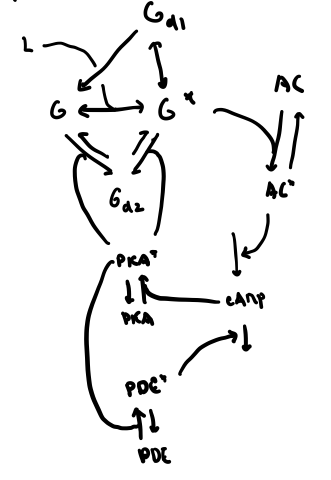
\includegraphics[width=0.4\linewidth]{Gd2_full_path.png}
	\centering
	\caption{Full model diagram from \cite{violin2008beta2}. Notation is changed from their paper to be more inline with ours, although this slightly changes the $G_{d1}$ desensitization pathway.}
	\label{fig:Gd2_full_model}
\end{figure}

\subsection{The New Model with $G_{d2}$}

Because it is unclear how exactly it would be best to model the complex downstream signal pathway that leads to heterologous desensitization, we opt to use a phenomenological model. We add a downstream signal molecule labeled $\lambda$ which acts as a proxy for the signal cascade (if it helps, we can think of it roughly as PKA). $\lambda$ is developed by $G^*$, and then naturally degrades exponentially. Then both $G$ and $G^*$ are capable of being transformed into $G_{d2}$, which naturally degrades back to $G$. The thinking here is that the recovery of $G_{d2}$ is much slower than the decoupling of the GPCR and its ligand, thus when recovering will turn into $G$. A drawing of this system is given on the right side of Fig \ref{fig:Gd2_full_model}.

\begin{figure}[H]
	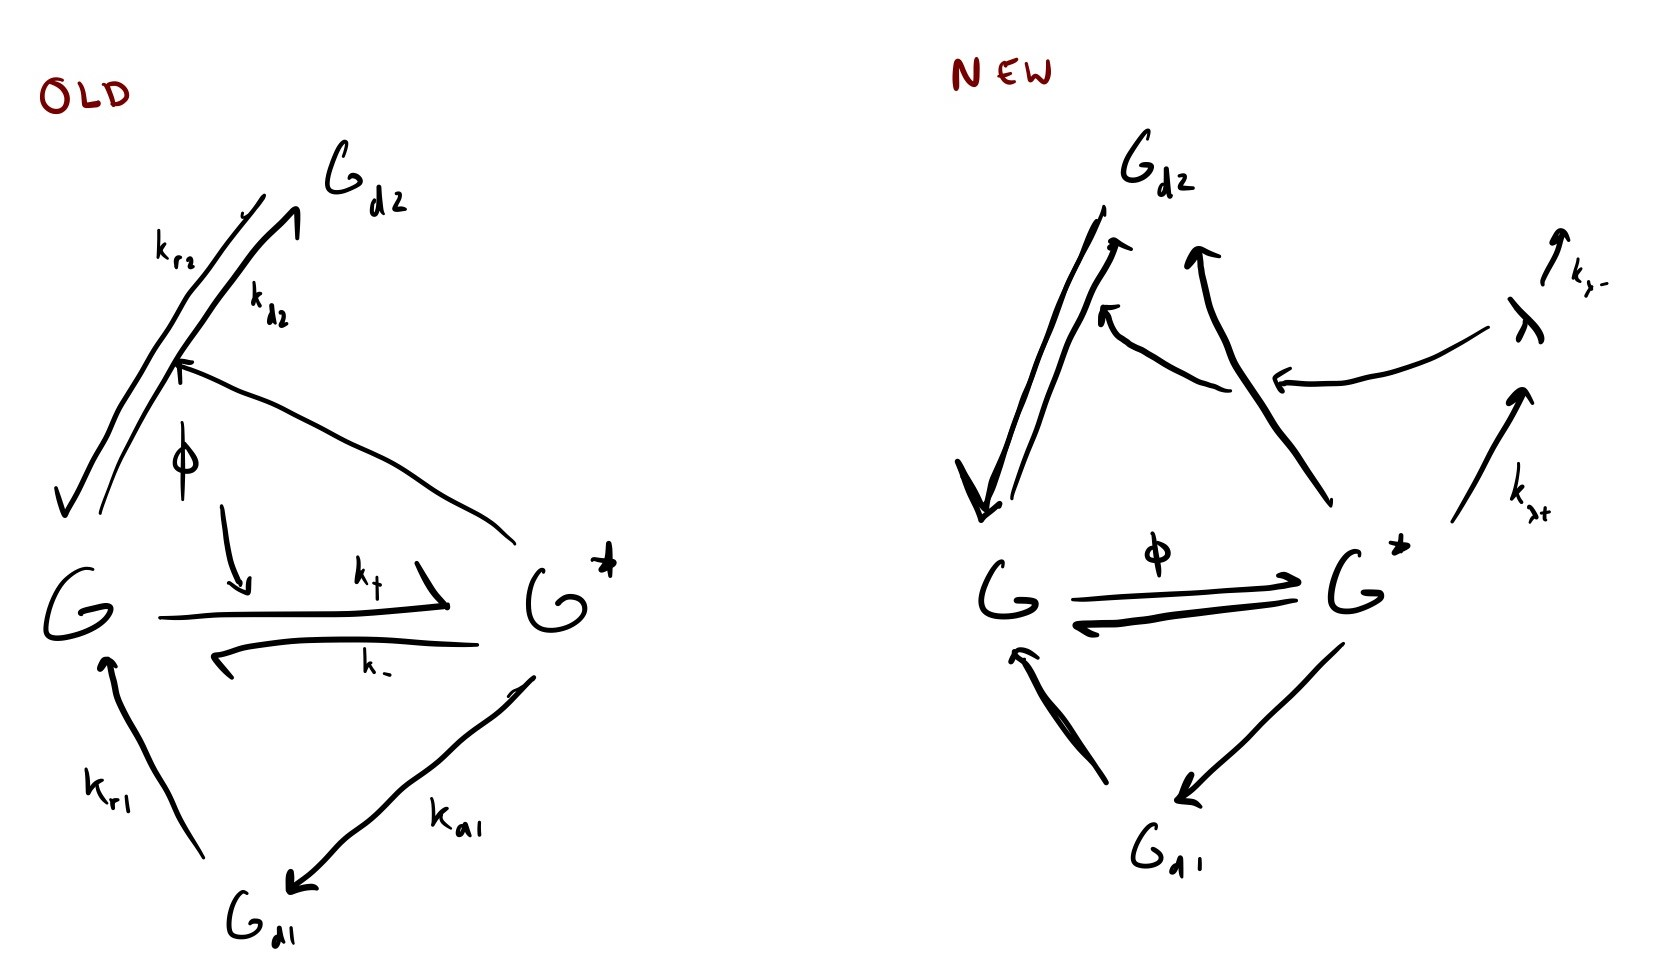
\includegraphics[width=0.7\linewidth]{new_GPCR_model.jpg}
	\centering
	\caption{Left: old model diagram. Right: new model diagram for glutamate GPCR including a downstream $G_{d2}$ activator $\lambda$}
	\label{fig:new_GPCR_model}
\end{figure}

The new dynamic equations are in total
\begin{align}
\frac{dG^*}{dt} &= k_+ \phi G - k_- G^* - k_{d1} G^* - k_{d2}\lambda G^*\\
\frac{dG_{d1}}{dt} &= k_{d1}G^* - k_{r1} G_{d1} \\
\frac{dG_{d2}}{dt} &= k_{d2}\lambda(G^*+G) - k_{r2} G_{d2} \\
\frac{d\lambda}{dt} &= k_{\lambda+}G^* - k_{\lambda-}\lambda
\end{align}
with $G = 1 - G_{d1} - G_{d2} - G^*$. An explanation of how parameter values were selected will be in the next section. A comparison of the bifurcation diagrams showing calcium oscillations with the full GPCR, IP3, Ca2+ model and glutamate as a bifurcation parameter is given in Fig \ref{fig:new_bifurcation}. In the previous model, $G_{d2}$ barely had any influence at all. It is clear that with the inclusion of $\lambda$ and the new parameter values, $G_{d2}$ is playing a significant role in desensitizing the GPCR, effectively decreasing the activation power of glutamate stimulation.

\begin{figure}[H]
	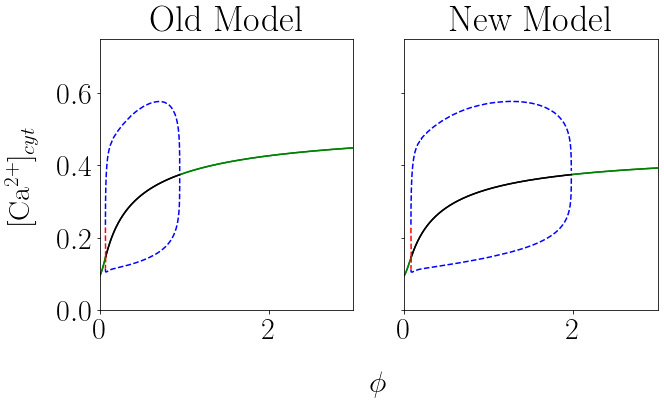
\includegraphics[width=0.7\linewidth]{c_glut_bifurcation_new.png}
	\centering
	\caption{Left: old bifurcation diagram. Right: new bifurcation diagram for full GPCR, IP3, Ca2+ model}
	\label{fig:new_bifurcation}
\end{figure}

\subsection{Fitting the New Model}

In order to pick a set of parameters, I tested a range of parameters on a set of double bath stimulation protocols. In these simulations, glutamate was given at concentrations of 0.1, 0.2, 0.5, and 1. Each of the two glutamate pulses lasted 30 seconds, with either 120, 240, or 600 seconds of no stimulation between them. Desensitization was measured as the ratio of max $G^*$ height attained during the second stimulation as compared to the first (which had a very strong correlation with the ratio of total $G^*$ integrated signal over the pulses). 

The parameters being modified were $k_{d1}, k_{r1}, k_{d2}, k_{r2}, k_{\lambda+}, k_{\lambda-}$ - in other words, those related to desensitization or to $\lambda$. From a base level of $k_{d1}=0.02, k_{r1}=0.01, k_{d2}=0.2, k_{r2}=0.005, k_{\lambda+}=0.0002, k_{\lambda-}=0.0004$, each of the parameters were either multiplied by 3, divided by 3, or left alone, leading to $3^6=729$ unique parameter combinations.

From here, I narrowed the search results to those with the following characteristics
\begin{itemize}
\item Noticeable desensitization with only 120 seconds of rest
\item Nearly full recovery with 600 seconds of rest
\item $G_{d2}$ having significantly slower timescale than $G_{d1}$
\item $G_{d2}$ having comparable magnitude as $G_{d1}$
\end{itemize}

From these conditions and the parameter sets tested, two were selected. Some of these simulation results are given in Fig \ref{fig:gpcr_param_gluts} and Fig \ref{fig:gpcr_param_times}. The primary parameter set is $k_{d1}=0.02, k_{r1}=0.01, k_{d2}=0.6, k_{r2}=0.005, k_{\lambda+}=0.0002, k_{\lambda-}=0.0004$, while the secondary is $k_{d1}=0.02, k_{r1}=0.03, k_{d2}=0.6, k_{r2}=0.005, k_{\lambda+}=0.0006, k_{\lambda-}=0.012$. Notably, the primary set has $G_{d1}$ and $G_{d2}$ with comparable strengths, but the secondary set has more complete recovery at 600 second rest times. However, in the secondary set, $\lambda$ has a time course which is more similar to $G_{d1}$, which may be undesirable.

\begin{figure}[H]
	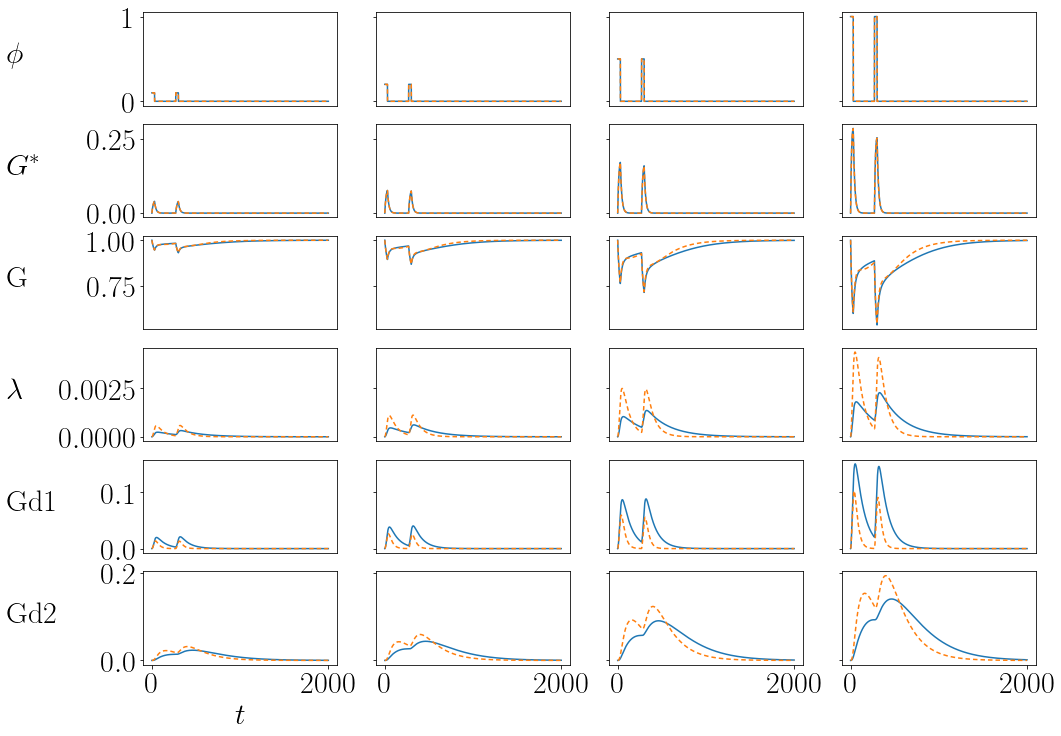
\includegraphics[width=1.0\linewidth]{figures/gpcr_param_gluts.png}
	\centering
	\caption{Double bath simulations with primary (solid, blue) and secondary (orange, dashed) parameter sets for GPCR, run at different glutamate levels}
	\label{fig:gpcr_param_gluts}
\end{figure}

\begin{figure}[H]
	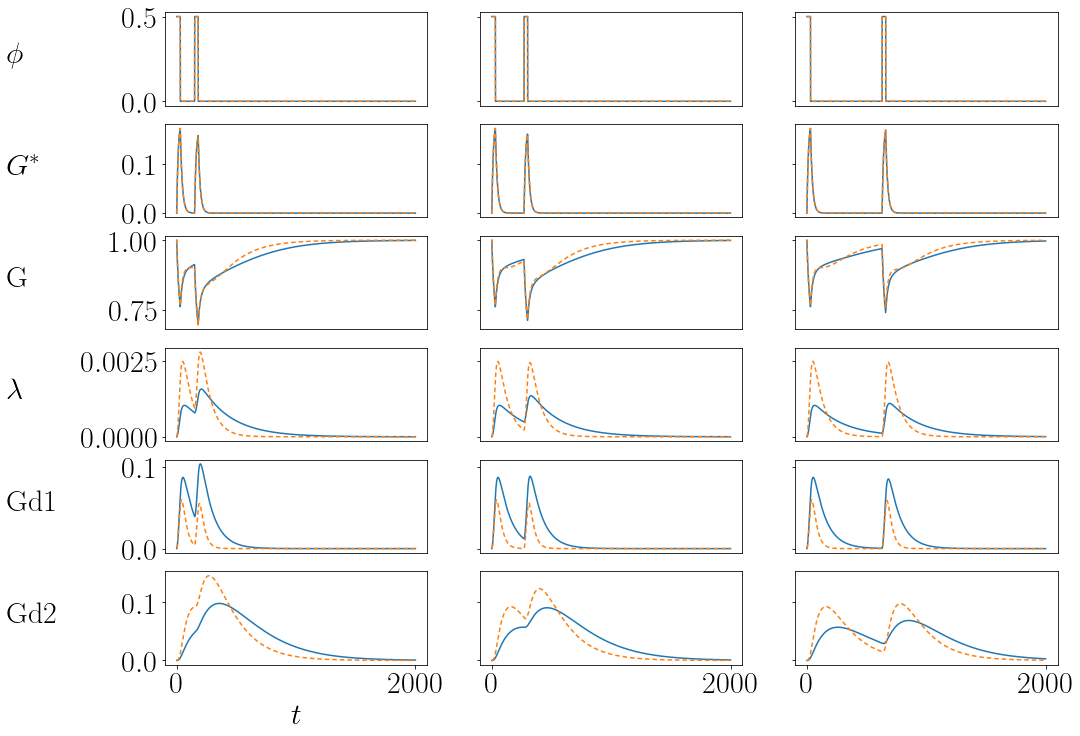
\includegraphics[width=1.0\linewidth]{figures/gpcr_param_times.png}
	\centering	
	\caption{Double bath simulations with primary (solid, blue) and secondary (orange, dashed) parameter sets for GPCR, run at glutamate strength of $0.5$ and different time between baths}
	\label{fig:gpcr_param_times}
\end{figure}

\subsection{New Full Model Properties}

We now apply this new GPCR model with the full IP3, Ca2+ dynamics. In the long bath experiment (Fig \ref{fig:full_pulse_comparison}), we note that the new model decreases the delay in calcium reaches its oscillation regime (this is more apparent for larger concentrations of glutamate, not shown). It is also clear that because $G_{d2}$ is much stronger than previously, $G^*$ is activated less strongly with the new model, and there is clear longer term desensitization that grows over time. In this long bath experiment, the two parameter sets begin to drift in oscillation frequency of calcium, as over a long period of time, the primary parameter set experience s slightly more desensitization.

In the double bath experiment (Fig \ref{fig:full_double_bath_comparison}), there appears to be little qualitative difference between the responses. In the spritz experiment (Fig \ref{fig:full_spritz_comparison}), we can see complicated calcium dynamics, which may be due to the feedback relation between calcium and IP3 (as the IP3 trace also does not look very smooth). 

Overall, it appears that the new model does predict slightly different dynamics to the old one, and that the two parameter sets lead to quantitatively similar calcium traces for more experimentally relevant protocols (and certainly for low total amount of glutamate stimulation).

\begin{figure}[H]
	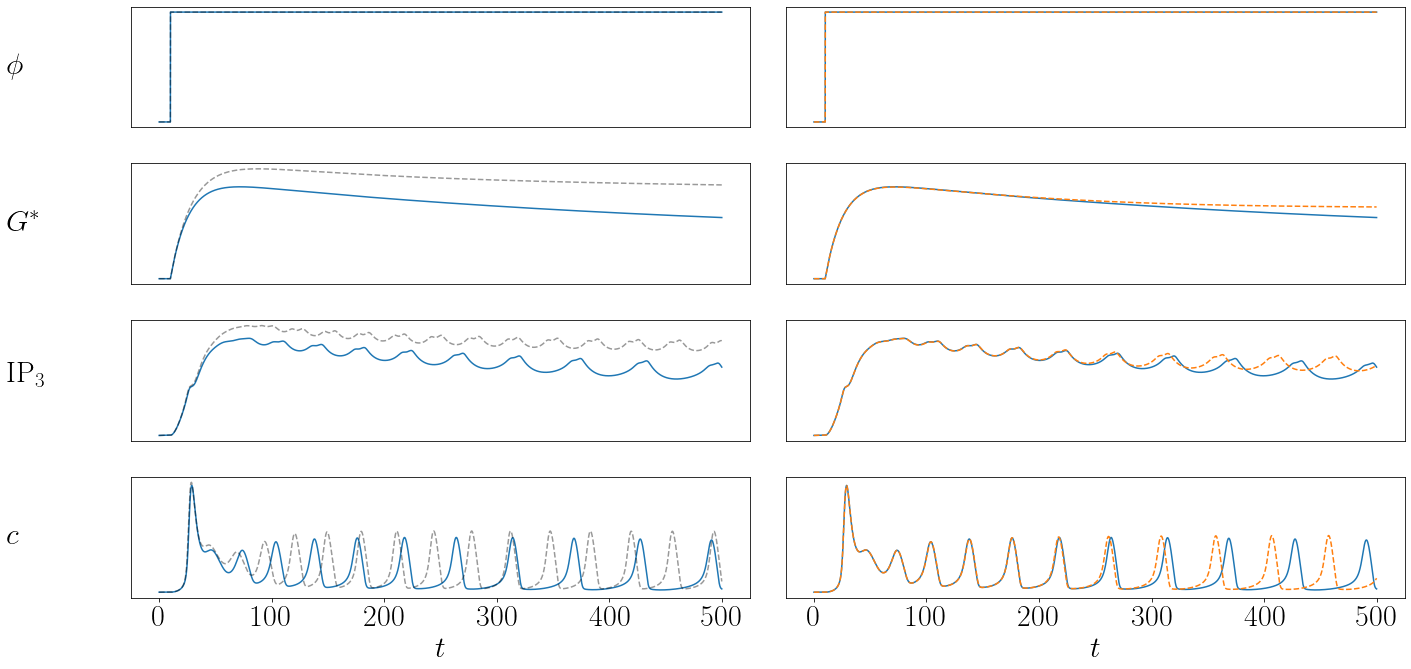
\includegraphics[width=1\linewidth]{figures/full_pulse_comparison.png}
	\centering
	\caption{Comparison of old model (grey, dashed) with new model primary parameter set (blue, solid) and secondary parameter set (orange, dashed) with long bath of glutamate input (0.15$\mu$M).}
	\label{fig:full_pulse_comparison}
\end{figure}

\begin{figure}[H]
	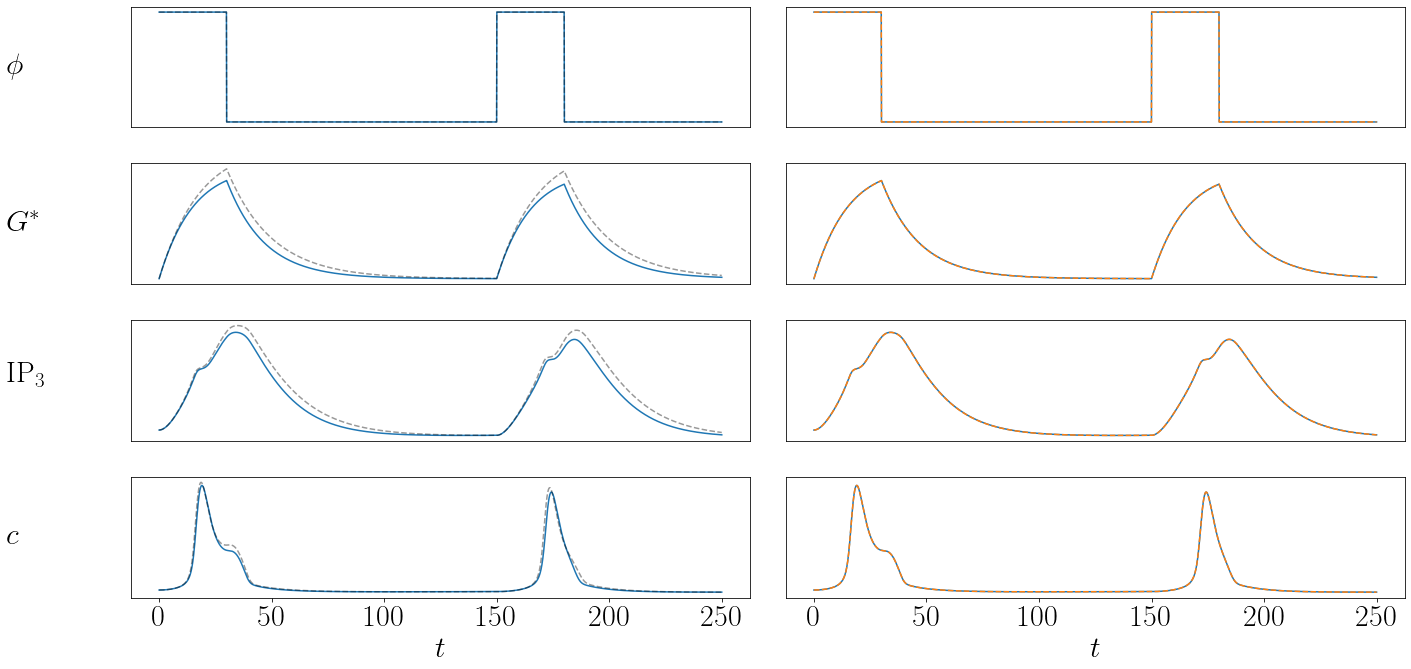
\includegraphics[width=1\linewidth]{figures/full_double_bath_comparison.png}
	\centering
	\caption{Comparison of old model (grey, dashed) with new model primary parameter set (blue, solid) and secondary parameter set (orange, dashed) with double bath of glutamate input (0.15$\mu$M, 30 seconds on, 120 seconds off).}
	\label{fig:full_double_bath_comparison}
\end{figure}

\begin{figure}[H]
	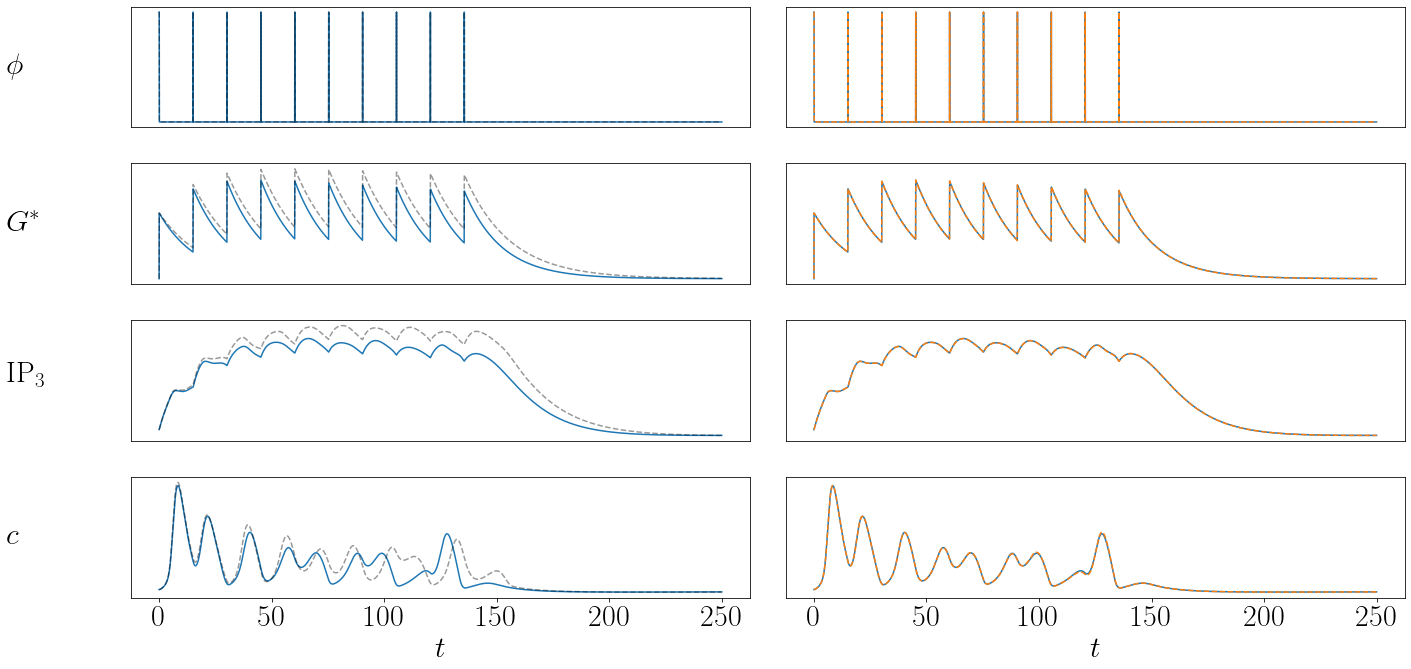
\includegraphics[width=1\linewidth]{figures/full_spritz_comparison.png}
	\centering
	\caption{Comparison of old model (grey, dashed) with new model primary parameter set (blue, solid) and secondary parameter set (orange, dashed) with spritz glutamate inputs (50$\mu$M, 60ms per spritz, 15 seconds between spritzes).}
	\label{fig:full_spritz_comparison}
\end{figure}


\subsubsection{Potential Problem with the Primary Parameter  Set}
In Fig \ref{fig:full_double_bath_comparison2} we perform the double bath experiment again, but this time show $G_{d1}$ and $G_{d2}$ as well. One worrying thing is that for the primary set $G_{d2}$ continues to grow for a significant period of time after the stimulation ends. This may be desirable behavior, but it may also be something to avoid.

\begin{figure}[H]
	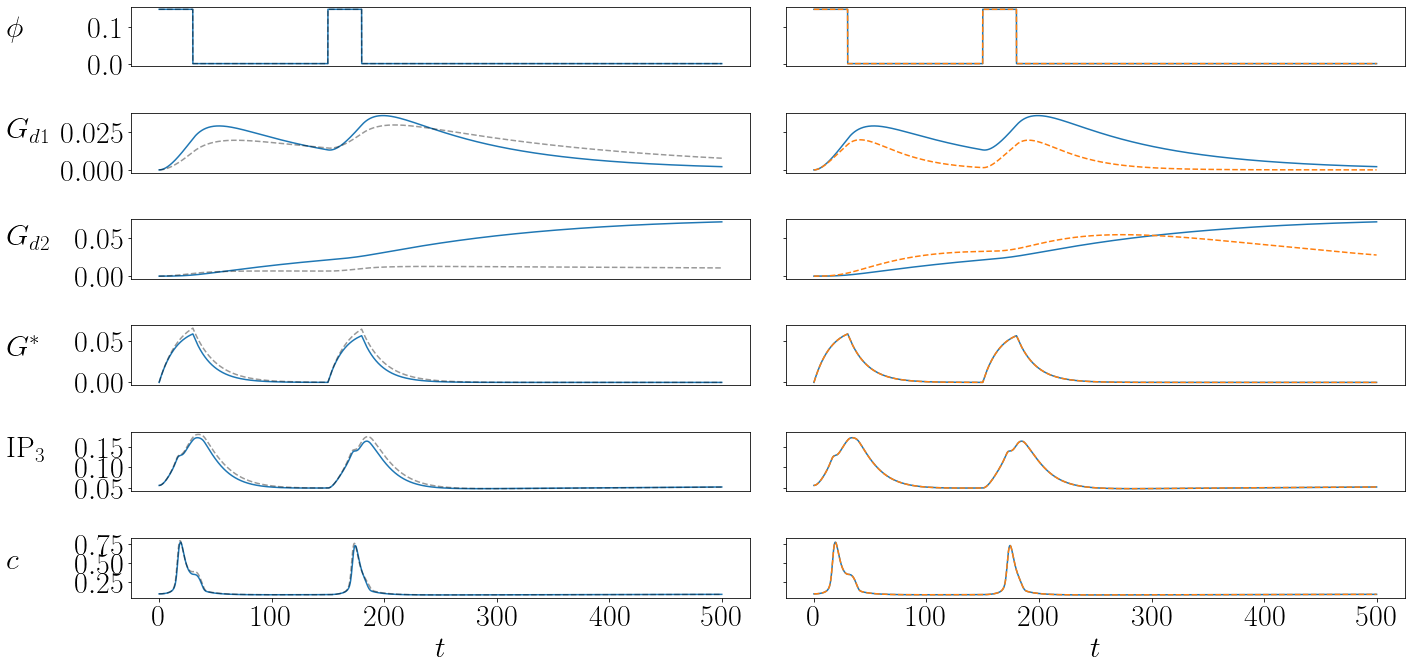
\includegraphics[width=1\linewidth]{figures/full_double_bath_comparison2.png}
	\centering
	\caption{Comparison of old model (grey, dashed) with new model primary parameter set (blue, solid) and secondary parameter set (orange, dashed) with double bath of glutamate input (0.15$\mu$M, 30 seconds on, 120 seconds off).}
	\label{fig:full_double_bath_comparison2}
\end{figure}


\subsection{Classifying Calcium Response}

In the previous progress update, we mentioned that Marsa identified four types of calcium response. Using the new system including IP3 and the GPCR dynamics, we would like to see if we can reproduce these four calcium responses for a range of glutamate inputs. First, I reproduced the calcium response classification code in Python, and the results of attempting to reproduce Figure 4 from \cite{taheri2017diversity} are shown in Fig \ref{fig:ip3_classification}. Notably, not all of the responses are classified in the same way as the original paper. Examples of how the calcium traces are classified algorithmically are given in Fig \ref{fig:glut_classification_examples}. 

\begin{figure}[H]
	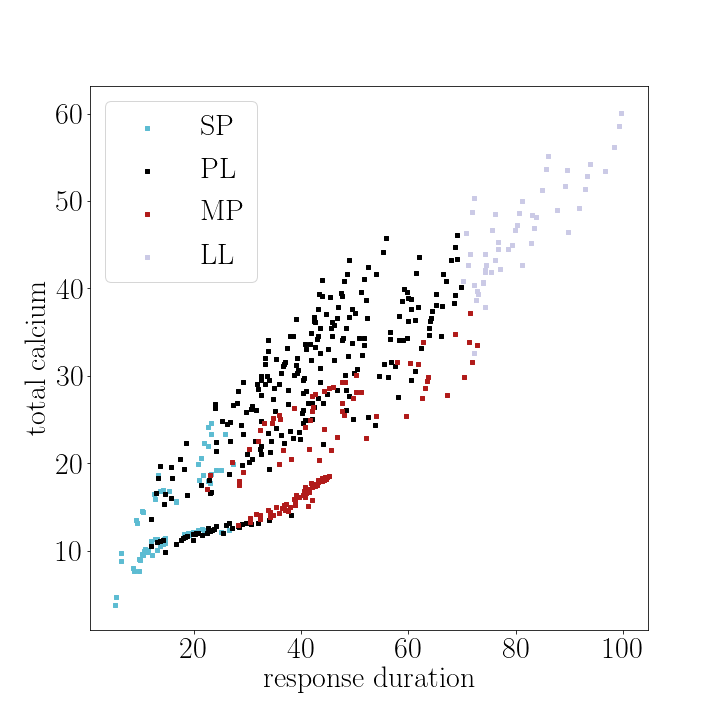
\includegraphics[width=0.6\linewidth]{ip3_classification.png}
	\centering
	\caption{Reproduction of Figure 4 from \cite{taheri2017diversity} using rewritten Python code. }
	\label{fig:ip3_classification}
\end{figure}

\begin{figure}[H]
	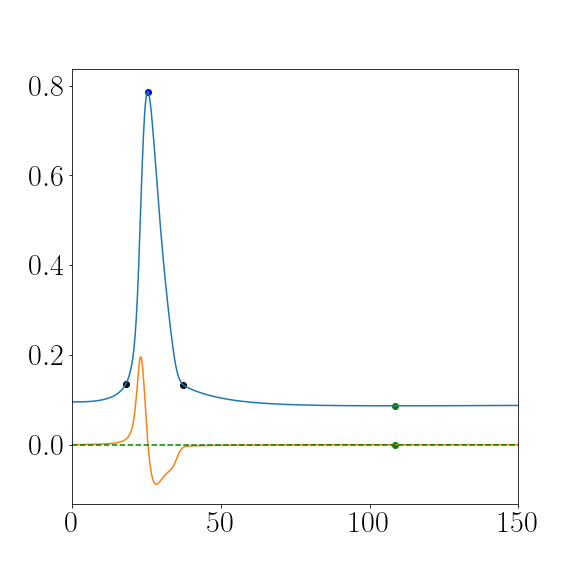
\includegraphics[width=0.3\linewidth]{SP_example.png}
	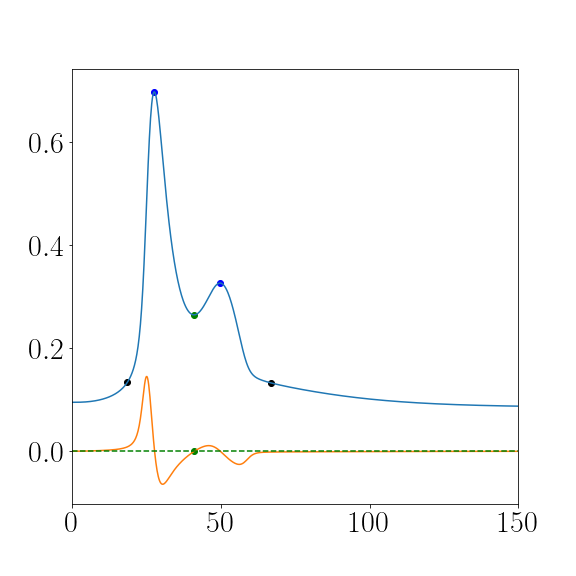
\includegraphics[width=0.3\linewidth]{MP_example.png}
	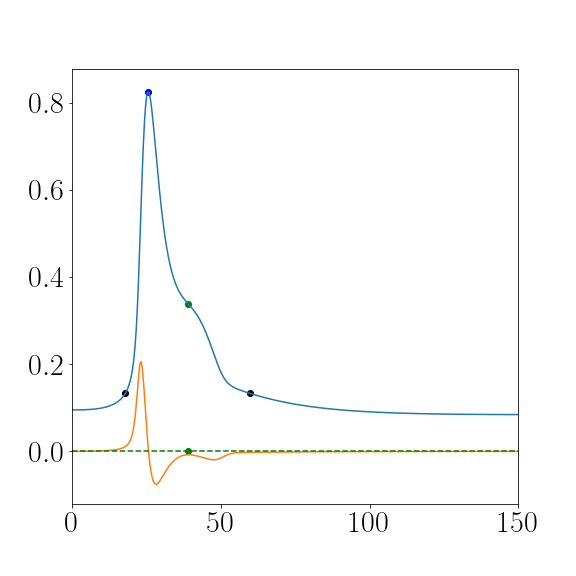
\includegraphics[width=0.3\linewidth]{PL_example.png}
	\centering
	\caption{Examples of calcium responses with the full dynamical system. Blue shows the calcium response, while orange shows the derivative of calcium. Scatter points label where algorithm divides different peak responses.}
	\label{fig:glut_classification_examples}
\end{figure}

In the previous progress report, we attempted to recreate this plot using the full dynamical system, giving glutamate double exponential pulses as inputs (Fig \ref{fig:glut_classification} left). We saw a problem where there were no responses classified as MP. Examining a number of cases, it seemed that the center trough in a lot of examples did not reach down low enough to classify as a ``true'' trough. This was likely due to the delay in reach oscillation caused by the inclusion of the calcium to IP3 negative feedback. 

Once again, we generated this classification plot using the new GPCR model this time. Here, we did have a few MP classifications, although fewer than the original Marsa paper. This agrees with our earlier findings that the new GPCR seems to decrease the amount of delay until calcium oscillation begins.

\begin{figure}[H]
	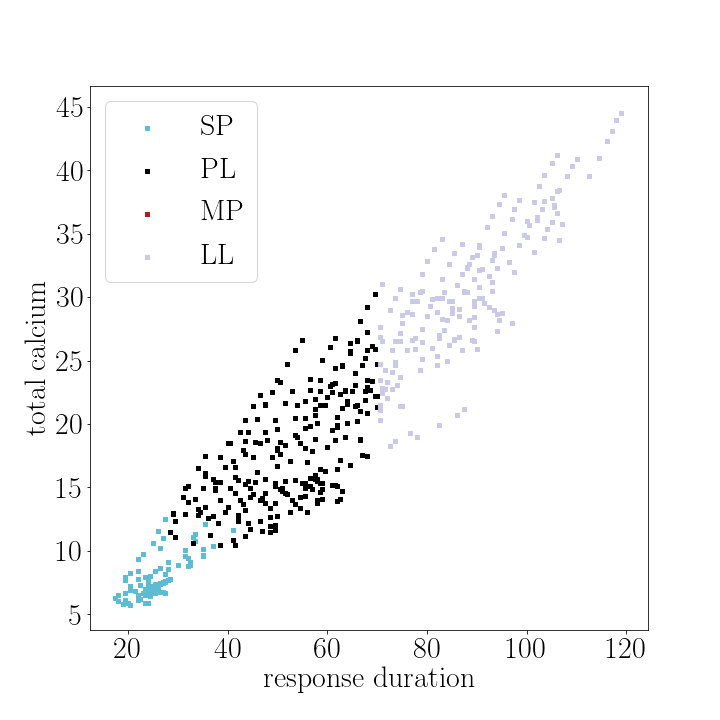
\includegraphics[width=0.45\linewidth]{glut_classification.png}
	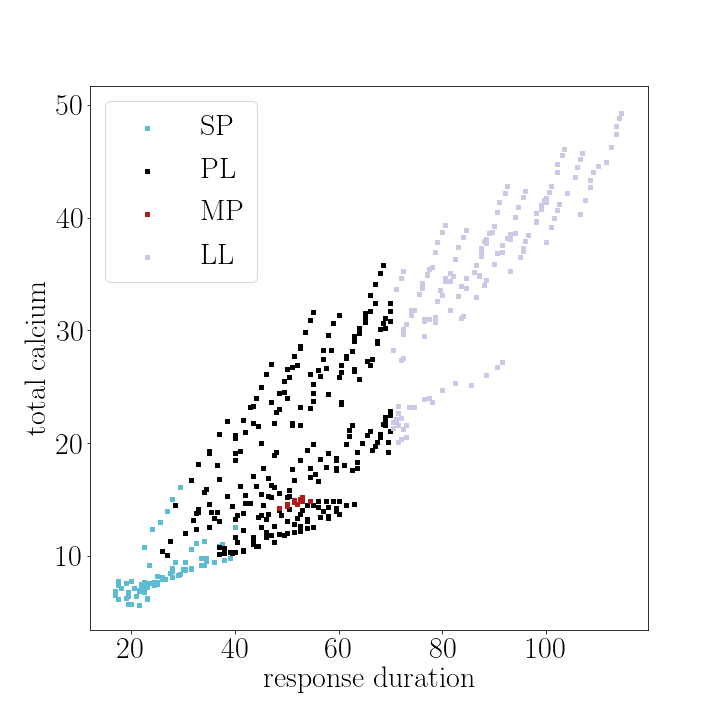
\includegraphics[width=0.45\linewidth]{glut_classification_new2.png}
	\centering
	\caption{Classification of responses for a range of glutamate double exponential curves. Left: full model with old GPCR. Right: full model with new GPCR. Note that for the new GPCR, glutamate traces have doubled amplitude as compared to \cite{taheri2017diversity} in order to make the total calcium generated more comparable.}
	\label{fig:glut_classification}
\end{figure}

\begin{figure}[H]
	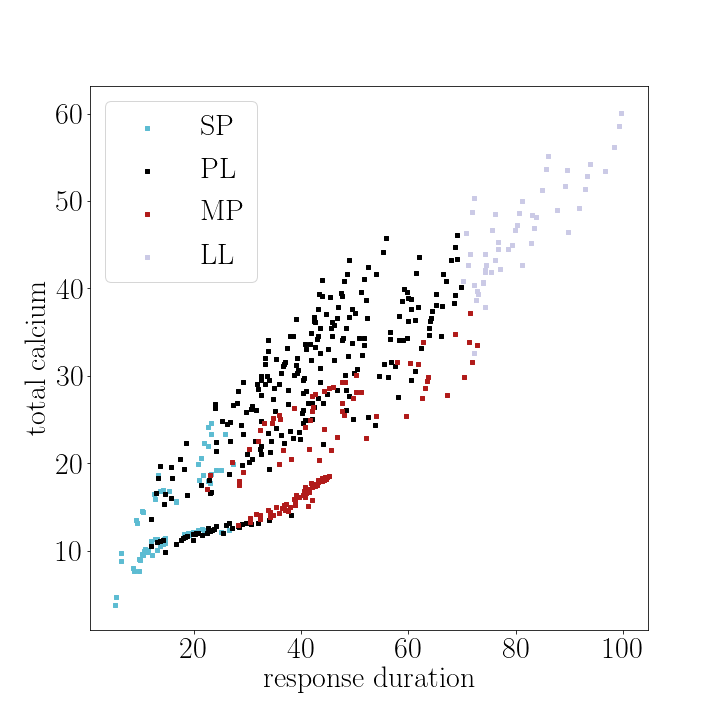
\includegraphics[width=0.45\linewidth]{ip3_classification.png}
	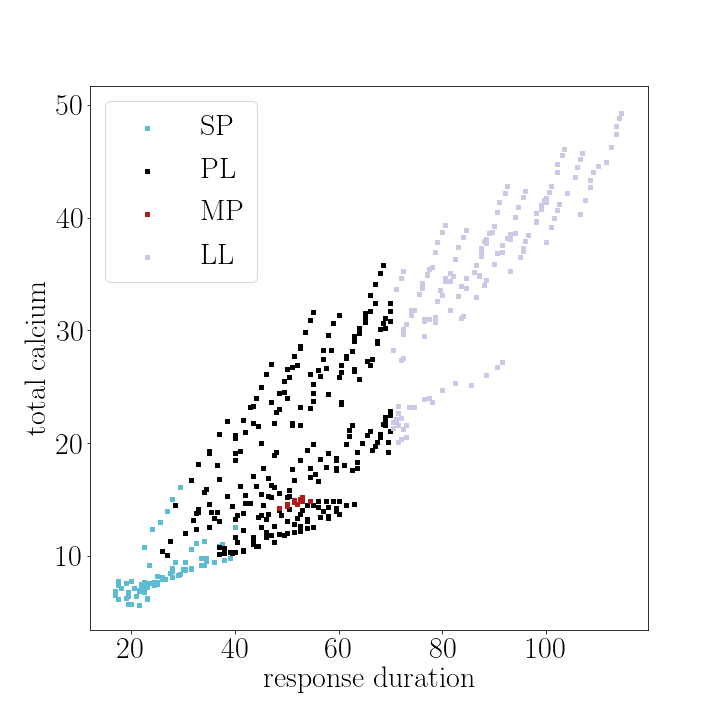
\includegraphics[width=0.45\linewidth]{glut_classification_new2.png}
	\centering
	\caption{Comparison of the classification plot using IP3 as an input, as in Marsa's paper (left) with the new GPCR model taking glutamate as an input (right)}
	\label{fig:glut_classification_2}
\end{figure}

\pagebreak

\bibliography{references}
\bibliographystyle{ieeetr}

\end{document}